\documentclass{beamer}
%
% Choose how your presentation looks.
%
% For more themes, color themes and font themes, see:
% http://deic.uab.es/~iblanes/beamer_gallery/index_by_theme.html
%

\setbeamertemplate{itemize/enumerate body begin}{\small}
\mode<presentation>
{
  \usetheme{default} % or try Darmstadt, Madrid, Warsaw, ...
  \usecolortheme{default} % or try albatross, beaver, crane, ...
  \usefonttheme{serif} % or try default, structurebold, ...
  \setbeamertemplate{navigation symbols}{}
  \setbeamertemplate{caption}[numbered]
}
\newcommand*\vf[1]{\mathbf{#1}}
\usepackage[english]{babel}
\usepackage[utf8x]{inputenc}
\usepackage{amsmath,mathtools,esint,bm}
\usepackage{todonotes}
\usepackage{blindtext}
\usepackage[font=scriptsize]{caption}
\usepackage[version=3]{mhchem}
\newcommand{\mick}[1]{\textcolor{red}{#1}}

\AtBeginSection[]{
  \begin{frame}
  \vfill
  \centering
  \begin{beamercolorbox}[sep=8pt,center,shadow=true,rounded=true]{title}
    \usebeamerfont{title}\insertsectionhead\par%
  \end{beamercolorbox}
  \vfill
  \end{frame}
}

\title[]{Thermal properties of a quantum critical point in hole-doped cuprates}
\author{Mick Krongchon}
\institute{University of Illinois at Urbana-Champaign}
\date{\today}

\begin{document}

\begin{frame}
\titlepage
\end{frame}
% Hi everyone, today I'm gonna talk about what we can learn from quantum critical point in cuprate superconductors from measuring specific heat
% From last time, we looked into charge density wave vector on doping.
% What quantities can we look into across a wide range of doping?
% One of these quantities is the specific heat because it can be accurately measured.

% \begin{frame}
% \centering
% \textit{intentionally left blank}
% \end{frame}

\begin{frame}{Outline}
\begin{itemize}
\item Background on quantum critical point
\item Thermal properties
\item Experiments on cuprates
\end{itemize}
\end{frame}
% This is my outline for this presentation

\begin{frame}{What is a quantum critical point (QCP)?}
\begin{itemize}
\item A 2nd-order phase transition at zero $T$ varying other parameters, such as doping or a magnetic field
\item A QCP under the superconducting dome is crucial to understand the high-$T_c$ superconductivity
\item In iron-based and heavy-fermion compounds, the AFM ends at the QCP
\item This is not the case for cuprates
\end{itemize}
\end{frame}
% it's a phase transition that occurs at absolute zero temperature when we change non-thermal parameters like doping or magnetic field
% a classical phase transition occurs because of thermal fluctuations
% but zero T, there's no thermal fluctuation, we call this nonthermal transition quantum phase transition, which is driven by quantum fluctuation, which has something to do with the uncertainty principle
% so a quantum critical point is basically the point that separates two quantum phases at zero T
% it was a question before whether the QCP lies within the SC dome. but recent reports kinda show that this is true
% and investigating this quantum critical point under the superconducting dome might help us understand more about high-temperature superconductors
% there's been evidence that the anti-ferromagnetic phase ends at the quantum critical point in iron-based and heavy-fermon materials.
% but there is report of such things in cuprates. this is what this paper talks about

\begin{frame}{Thermodynamic signature of a QCP is a diverging electronic mass}
\begin{itemize}
\item For an AFM QCP,
\begin{align}
C_{\text{el}}/T \propto m^{\ast} \propto \log{(1/|x - x^{\ast}|)},
\end{align}
where $x$ is a non-thermal parameter
\item At $x = x^{\ast}$, we expect that $C_{\text{el}}/T \propto \log{(1/T)}$
\item In YBCO, $m^{\ast}$ increases as $p$ approaches $p^{\ast}$ suggesting that $p^{\ast}$ might be a QCP\footnotemark
\item To conclude a QCP, we need to measure the normal-state specific heat of a cuprate
\end{itemize}
\footnotetext[1]{Ramshaw, B. J. et al. Science 348, 317–320 (2015)}
\end{frame}
% For anti-ferromagnetic phase, we expect the mass and C/T to be proportional to log of one over the distance from a non-thermal parameter to the quantum critical point
% I don't think this statement is trivial at all.
% This behavior was observed in YBCO by Ranshaw et al 2015 but instead of at an anti-ferromagnetic phase, at a pseudogap phase
% We can't conclude that until we directly measure the specific heat of the normal-state cuprates as T goes to zero
% And this is what they did

\begin{frame}{Measuring the specific heat of cuprates}
\begin{itemize}
\item $C(T)$ was measured in La$_{1.8 - x}$Eu$_{0.2}$Sr$_{x}$CuO$_4$ (Eu-LSCO) and La$_{1.6 - x}$Nd$_{0.4}$Sr$_x$CuO$_4$ (Nd-LSCO)\footnotemark
\begin{figure}
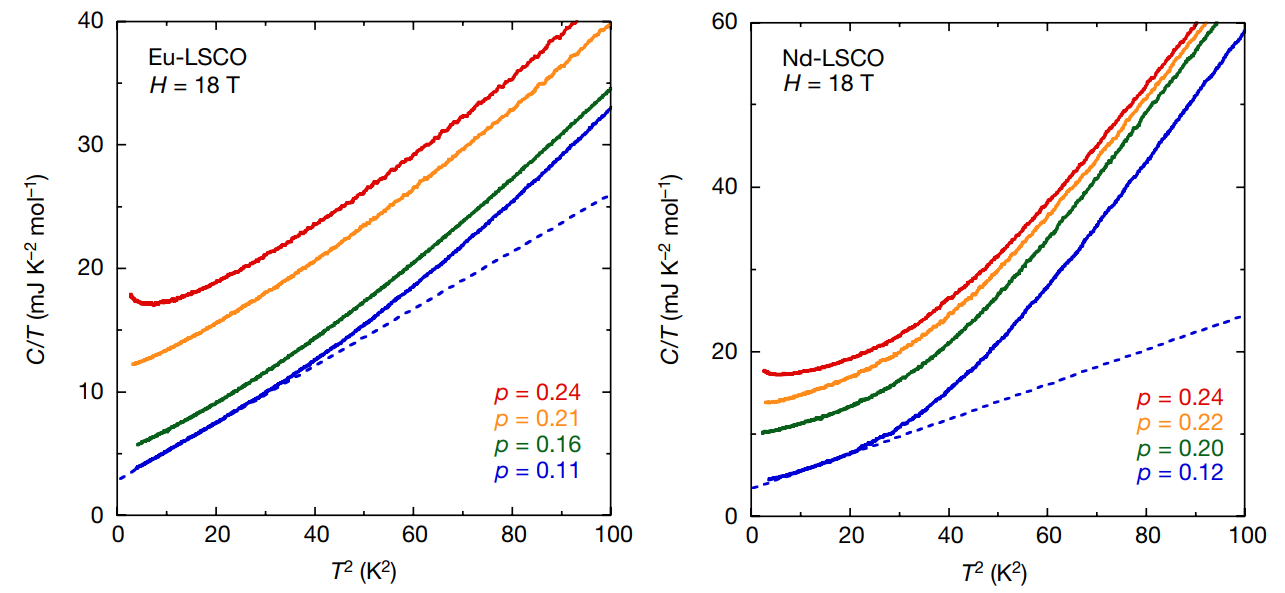
\includegraphics[width=3in]{figs/c_raw.png}
\caption*{Specific heat $C = C_{\text{el}} + C_{\text{ph}}$ of Eu-LSCO and Nd-LSCO}
\end{figure}
\item H = 18 T shifts the magnetic moment contribution, $C_{\text{mag}}$ to higher $T$ (Schottky effect)
\item The data obey $C/T = \gamma + \beta T^2$ at $T < 5~\rm{K}$ below $p \approx 0.20$
\end{itemize}
\footnotetext[2]{Michon, Bastien, et al. Nature 567.7747 (2019): 218}
\end{frame}
% This work was published by Michon et al last month.
% They measured the specific heat on various dopings of two cuprates.
% The result is shownn in these plots
% The two materials actually lose superconductivity at 8 T because we want to measure the specific heat at the normal state
% but they cranked the magnetic field up to 18 T to shift away the magnetic moment effect so that there's no magnetic contribution at below 5 K
% This is called the Schottky effect
% And we can see that the data follow this expression at low temperature and low dopings

\begin{frame}{Higher dopings Nd-LSCO (now polycrystalline powder)}
\begin{itemize}
\item No longer superconducting
\item Cannot use a field to shift Schottky effect since the field effect is anisotropic on polycrystalline powder
\item $C_{\text{mag}}$ was present in the raw data
\begin{figure}
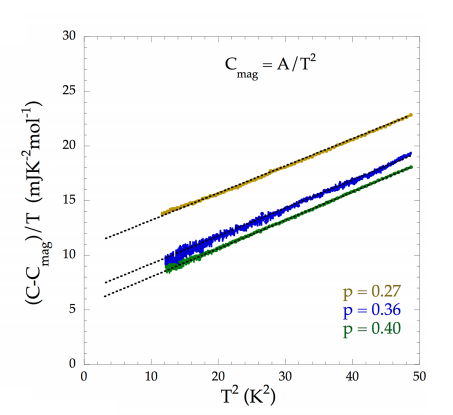
\includegraphics[width=2in]{figs/nd_high_dopings.png}
\caption*{Specific heat of the polycrystalline samples at p = 0.27, 0.36 and 0.40}
\end{figure}
\end{itemize}
\end{frame}
% Now for the higher dopings, I don't think they did any measurements on Eu-LSCO
% But they did it on Nd-LSCO using polycrystalline poweder samples because it's hard to grow single crystals at this high doping
% At this high doping, these samples are no longer superconducting.
% So there's no need to use a magnetic field to destroy superconductivity
% But they cannot use the field to shift away the Schottky effect either because it has an anisotropic effect on polycrystalline powder
% So, the magnetic contribution was present in the raw data but they subtracted it
% The way they did this is to measure magnetic contribution in both the single crystal and polycrystalline powder
% They found that C_mag is proportional to T^2. So, they used this information to fit the raw data and subtract the magnetic contribution from the raw data
% We see that the result follows the same expression = gamma + beta T^2

\begin{frame}{Thermal signature of the pseudogap critical point at $p^{\ast}$}
\begin{itemize}
\item $C_{\text{el}}$ is extracted and plotted vs. doping
\item Either van Hove singularity (vHs) or a QCP ($p_{\text{vHs}} \approx p^{\ast}$\footnotemark)
\begin{figure}
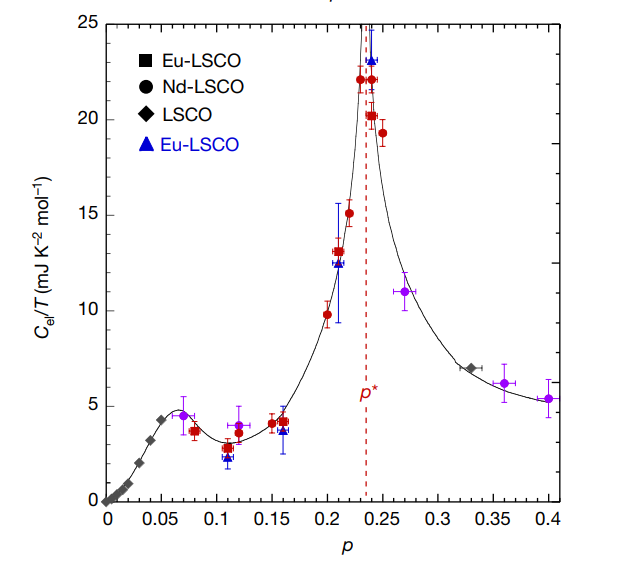
\includegraphics[width=2.1in]{figs/c_el_p.png}
\caption*{Doping dependence of the electronic specific heat. $p^{\ast} = 0.23(1)$\footnotemark}
\end{figure}
\end{itemize}
\footnotetext[3]{Matt, C. E. et al. Phys. Rev. B 92, 134524 (2015)}
\footnotetext[4]{Collignon, C. et al. Phys. Rev. B 95, 224517 (2017)}
\end{frame}
% So from here they did some more manipulation that involves subtracting data from a curve at a certain doping to extract the electronic contribution
% Now, we have already arrived at probably a grand conclusion of this paper, which is to say that there's a huge peak at p*,
% And we know p* comes from the another experiment here
% The explanation for this peak is either from vHs or a QCP
% We and know that there's indeed a vHs at the same spot as p* (is that a coincident?)

\begin{frame}{The band structure of Nd-LSCO is well-known}
\begin{itemize}
\item $C_{\text{el}}$ is calculated from the one-band tight-binding model
\footnotesize
\begin{align*}
\xi_k &= -\mu - 2t[\cos{(k_x a)} + \cos{(k_y b)}] - 4t^{\prime}\cos{(k_x a)}\cos{(k_y b)} \\
&~~~ -2t^{\prime\prime}\cos{(2k_x a)} \cos{(2k_y b)} \\
&~~~ -2t_z \cos{(k_z c / 2)}[\cos{(k_x a)} - \cos{(k_y b)}]^2 \cos{(k_x a / 2)} \cos{(k_y b / 2)}.\footnotemark \\
C_{\rm{el}}(T) &= \int_{-\infty}^{\infty} \frac{\partial f(\epsilon)}{\partial T} \epsilon N(\epsilon)~d\epsilon.
\end{align*}
\normalsize
\item The 3D character can be controlled by adjusting $t_z$
\end{itemize}
\footnotetext[5]{Markiewicz, R. S. et al. Phys. Rev. B 72, 054519 (2005)}
\end{frame}
% Luckily, the electronic specific heat due to band structure can be calculated using this one-band tight-binding model


\begin{frame}{The peak from vHs is small for the actual 3D dispersion}
\begin{itemize}
\item The sharp peak has to come from electronic effects beyond the band structure
\begin{figure}
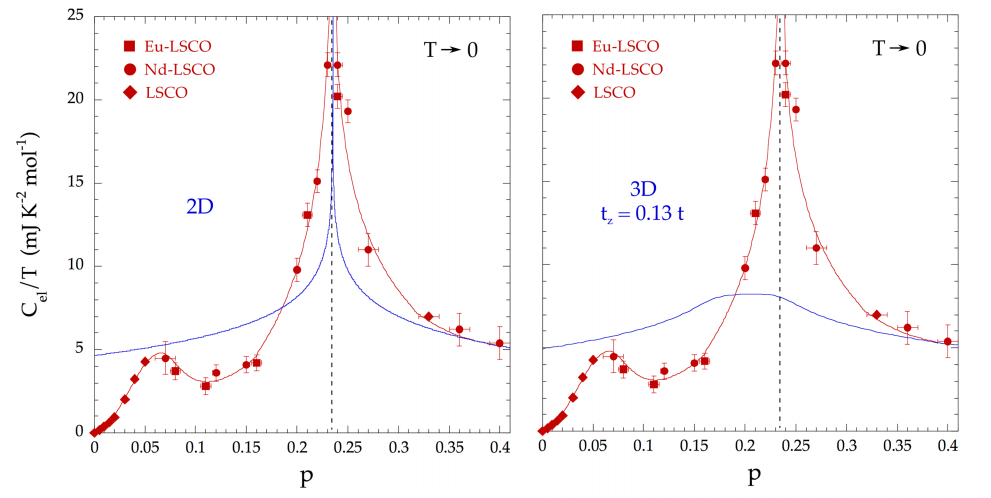
\includegraphics[width=3.5in]{figs/c_2d_vs_3d.png}
\caption*{Comparison of the measured specific heat and the calculation from the band structure}
\end{figure}
\end{itemize}
\end{frame}

\begin{frame}{$T$ dependence of $C_{\text{el}}$}
\begin{itemize}
\item At $p = 0.11$, $C_{\text{el}}/T$ is constant
\item At $p = 0.24$, $C_{\text{el}}/T \propto \log{(1/T)}$
\item Both Eu-LSCO and Nd-LSCO show the thermodynamic signature of a QCP
\item This was observed in AFM heavy-fermion metals
\begin{figure}
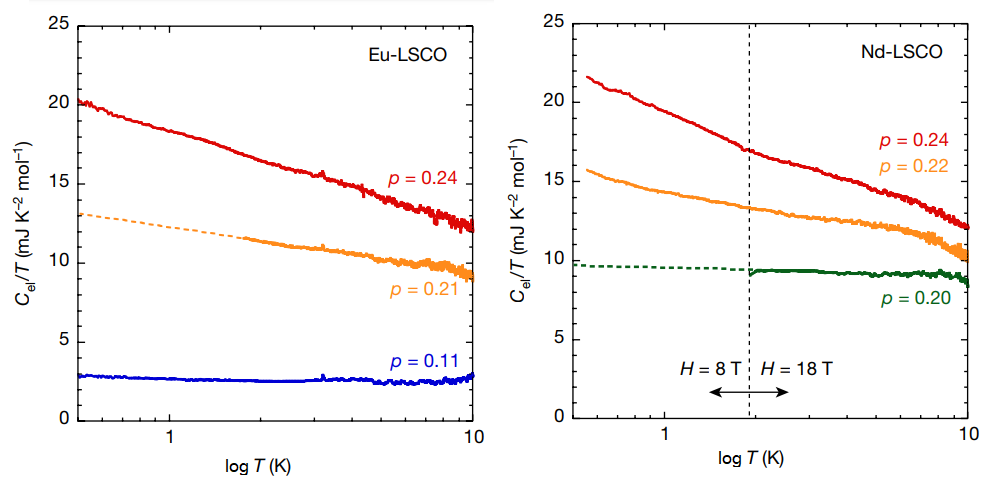
\includegraphics[width=3in]{figs/c_el.png}
\caption*{The electronic specific heat of Eu-LSCO and Nd-LSCO}
\end{figure}
\end{itemize}
\end{frame}

\begin{frame}{Summary}
\begin{itemize}
\item $C_{\text{el}}/T$ at $p^{\ast}$ peaks at $p^{\ast}$
\item $C_{\text{el}}/T \propto \log{(1/T)}$
\item Direct measurements of the specific heat in other normal-state hole-doped cuprates are needed
\end{itemize}
\end{frame}

% \begin{frame}{Goal: Mechanism for high-$T_\text{c}$ superconductivity (SC)}
% \begin{itemize}
% \item $T$ and magnetic field dependence show competition between charge density wave (CDW) and SC in YBCO by J. Chang et~al (2012)
% \end{itemize}
% \begin{figure}
% 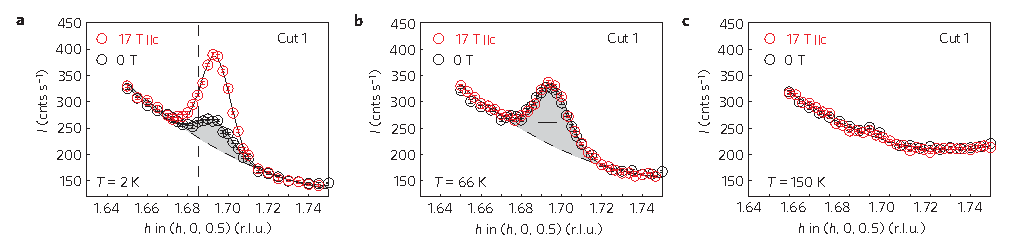
\includegraphics[width=\textwidth]{figs/chang_1.pdf}
% \caption*{Scans along $(h, 0, 0.5)$ for magnetic fields and temperature: \\(a) $T < T_c$, (b) $T_c < T < T_{\text{CDW}}$, (c) $T > T_{\text{CDW}}$}
% \end{figure}
% \end{frame}
% % We want to understand high temperature superconductivity
% % And last time, I showed the evidence of competition between CDW and SC in YBCO by J. Chang in 2012
% % So, just to recap: the CDW signal increases when SC is suppressed
% % But today we're gonna look into BSCCO because CDW is pretty common among cuprates, and doping in BSCCO can be tuned over a wide range

% \begin{frame}{CDW in the underdoped and optimally doped BSCCO}
% \begin{itemize}
% \item Y. Y. Peng et~al. (2016): RIXS for UD15K (p = 0.115) and OP33K (p = 0.16)
% \end{itemize}
% \begin{figure}
% 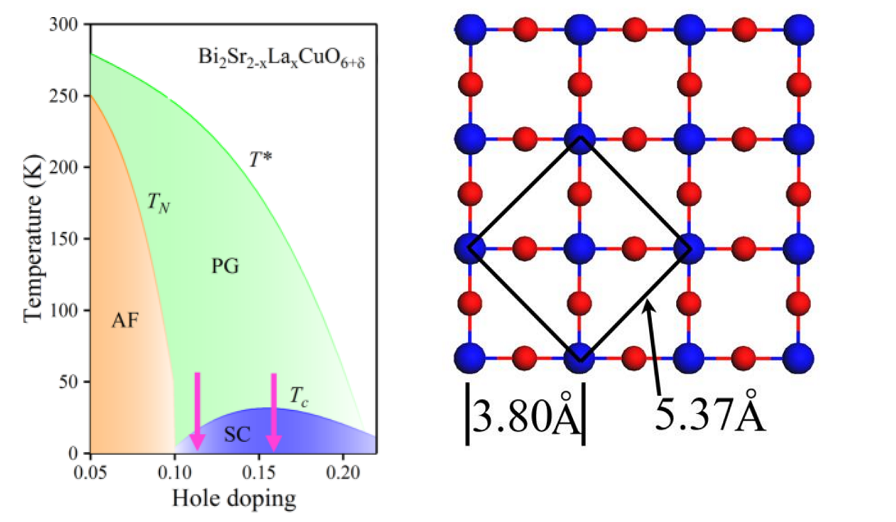
\includegraphics[width=3.5in]{figs/1a_lattice.png}
% \caption*{(\textbf{Left}) Phase diagram of Bi2201. (\textbf{Right}) Lattice image of the CuO$_2$ plane}
% \end{figure}
% \end{frame}
% % So, the experiment I want to talk about was done by Ying Ying Peng, who is now a post-doc from Peter Abbamonte group, and other people.
% % For Bi2201, previous RIXS results show no evidence of CDW at optimal doping (in contrast to the ARPES results)
% % That's another motivation to do this experiment
% % And, the two dopings that they did were UD15K, which is a shorthand for underdoped which has Tc = 15K, and OP33K

% \begin{frame}{CDW modulates only along Cu-O bonds}
% \begin{itemize}
% \item Find $q_\text{CDW}$ from RIXS energy/momentum intensity maps
% \item $q_\text{CDW} = 0.26$ for UD15K and $q_\text{CDW} = 0.23$ for OP33K
% \end{itemize}
% \begin{figure}
% 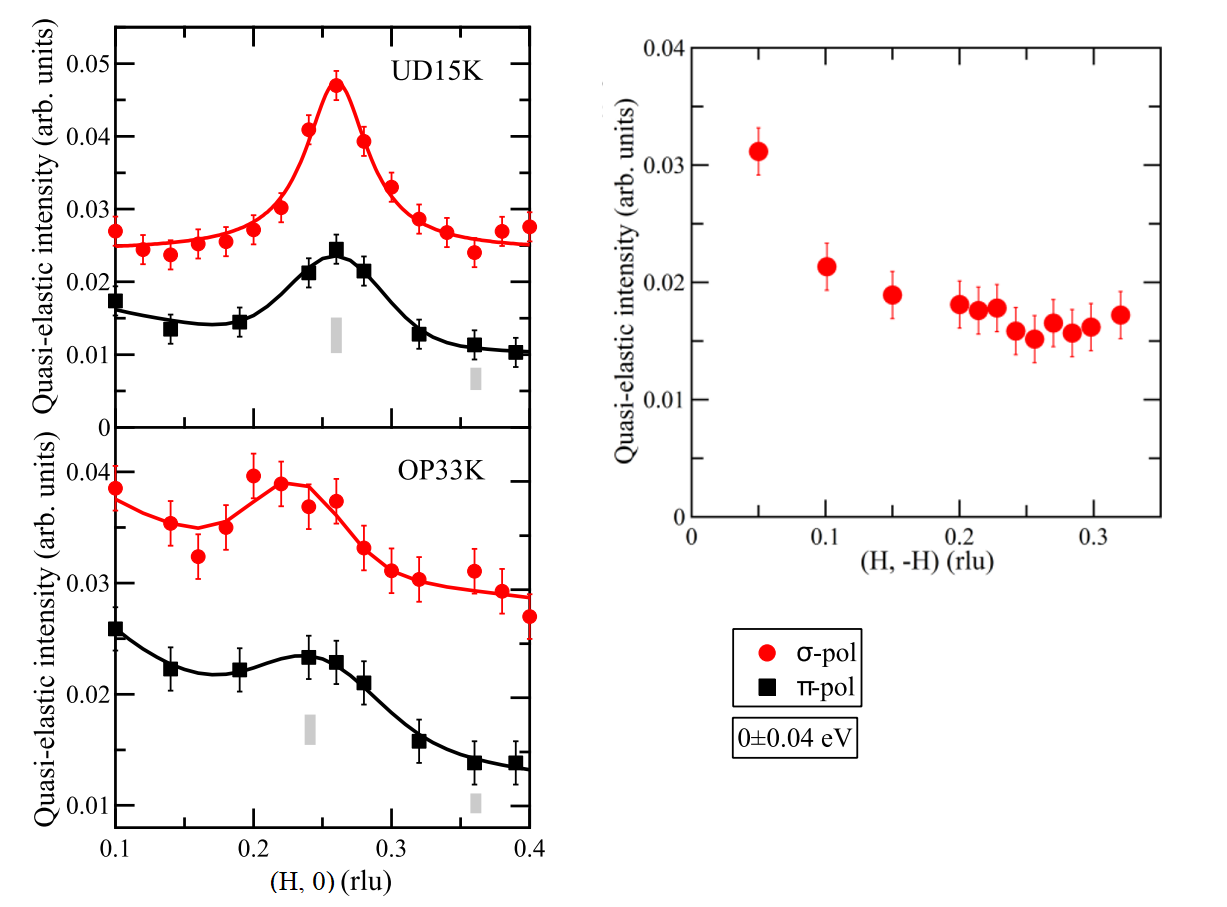
\includegraphics[width=3.2in]{figs/2ab_4a.png}
% \caption*{Intensity along (0,0)-(0.5,0) (\textbf{left}) and along (0,0)-(0.5,-0.5) (\textbf{right}) for UD15K}
% \end{figure}
% \end{frame}
% % So, when we do the RIXS experiment, we should get the energy/momentum intensity maps, which I do not show
% % And, from there, we can find q_CDW by analyzing the peaks from the cut, in this case E = 0 \pm 0.04 ev
% % On the left, we can see the peak, and they call this peak REXS
% % The intensity doesn't show any peak.
% % This confirms that CDW is only along Cu-O bonds.

% \begin{frame}{Temperature dependence}
% \begin{itemize}
% \item CDW signal can be seen at 20~K and becomes sharper at 33~K (similar to YBCO)
% \item Confirms the competition between CDW and SC
% \end{itemize}
% \begin{figure}
% 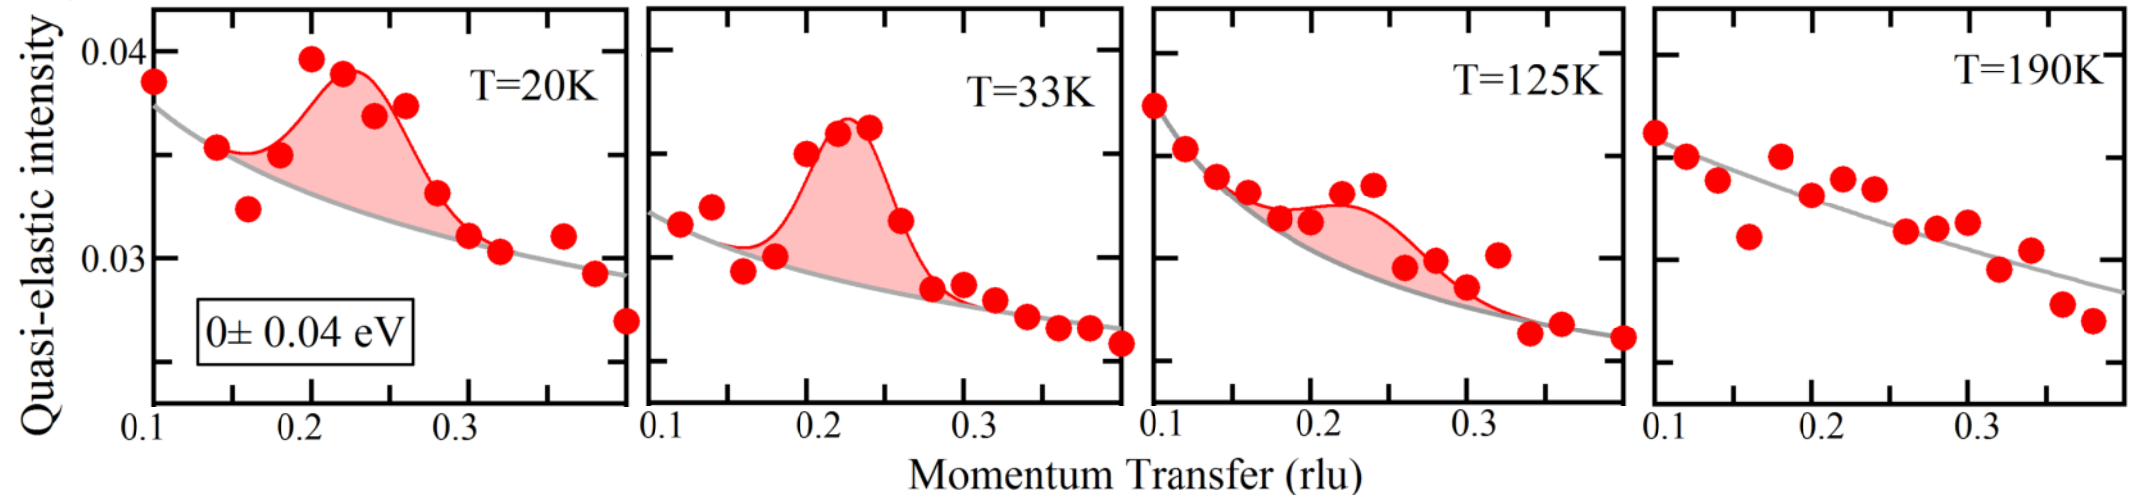
\includegraphics[width=4.2in]{figs/5e.png}
% \caption*{Temperature dependence across $T_c = 33~\mathrm{K}$ and $T^{*} = 160~\mathrm{K}$ for OP33K}
% \end{figure}
% \end{frame}


% \begin{frame}{What about the overdoped region?}
% \begin{itemize}
% \item No direct evidence of CDW in overdoped cuprates even though it was predicted in theory
% \item Y. Y. Peng et~al. (2018): RIXS for Bi2201 in OD17K ($p = 0.205$), OD11K ($p = 0.215$), and OD0K ($p = 0.23$)
% \end{itemize}
% \begin{figure}
% 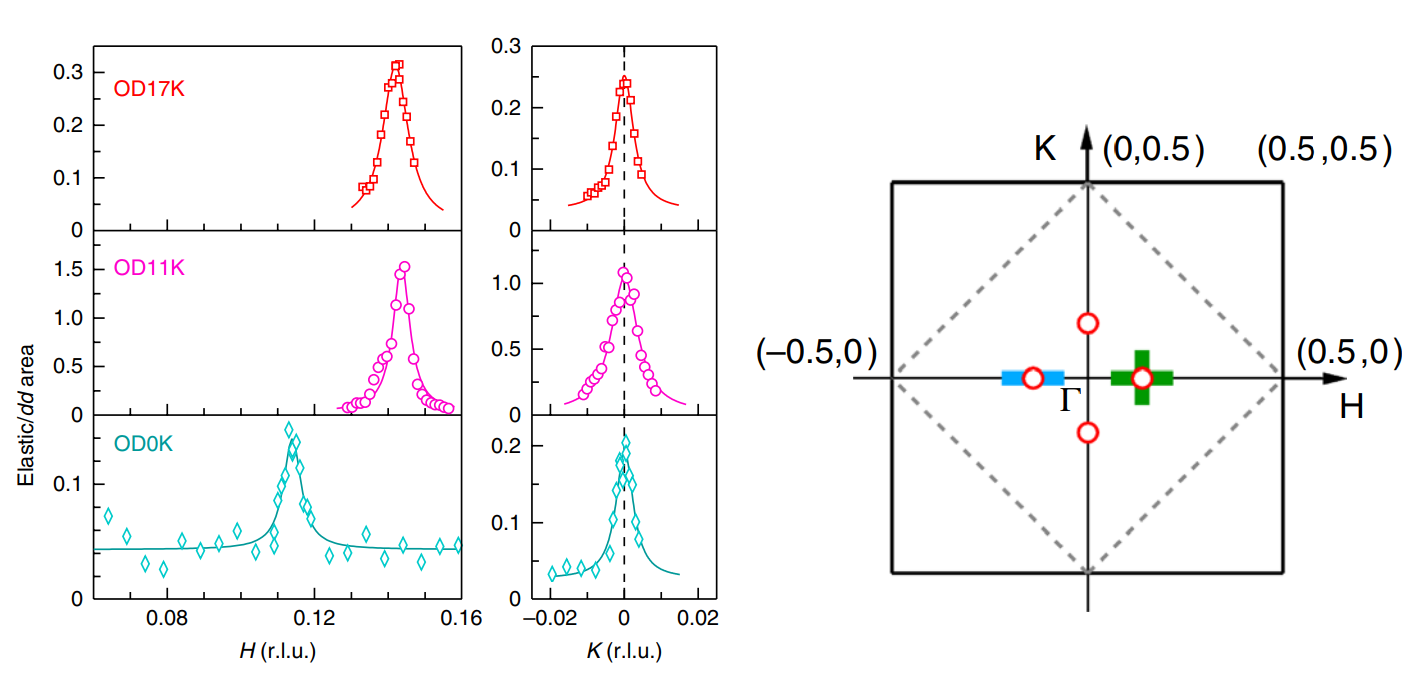
\includegraphics[width=4in]{figs/2018_2b.png}
% \caption*{REXS intensity along $H$ and $K$ at different doping levels}
% \end{figure}
% \end{frame}

% \begin{frame}{Small temperature dependence}
% \begin{itemize}
% \item CDW can still occur well above 250~K (even in the absense of the pseudogap)
% \end{itemize}
% \begin{figure}
% 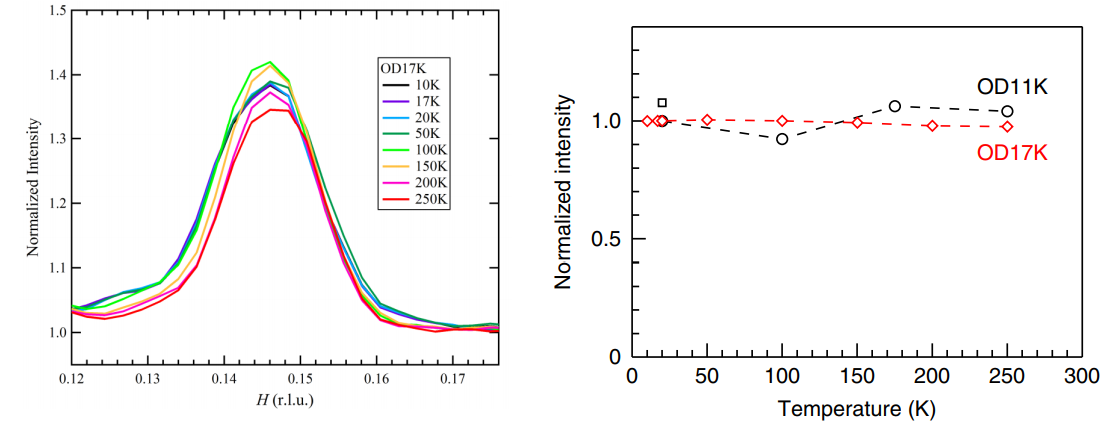
\includegraphics[width=4in]{figs/2018_s10_3d.png}
% \caption*{(\textbf{Left}) Intensity scans at different temperatures in OD17~K. (\textbf{Right}) Temperature dependence in OD11K and OD17K (normalized to at 20~K)}
% \end{figure}
% \end{frame}

% \begin{frame}{Do REXS peaks actually arise from CDW?}
% \begin{itemize}
% \item Charge scattering (no spin-flip) conserves the photon polarization
% \item Bi2201 has only one Cu site contributing to the x-ray absorption spectrum, and can be assigned to CDW in CuO$_2$ planes
% \end{itemize}
% \begin{figure}
% 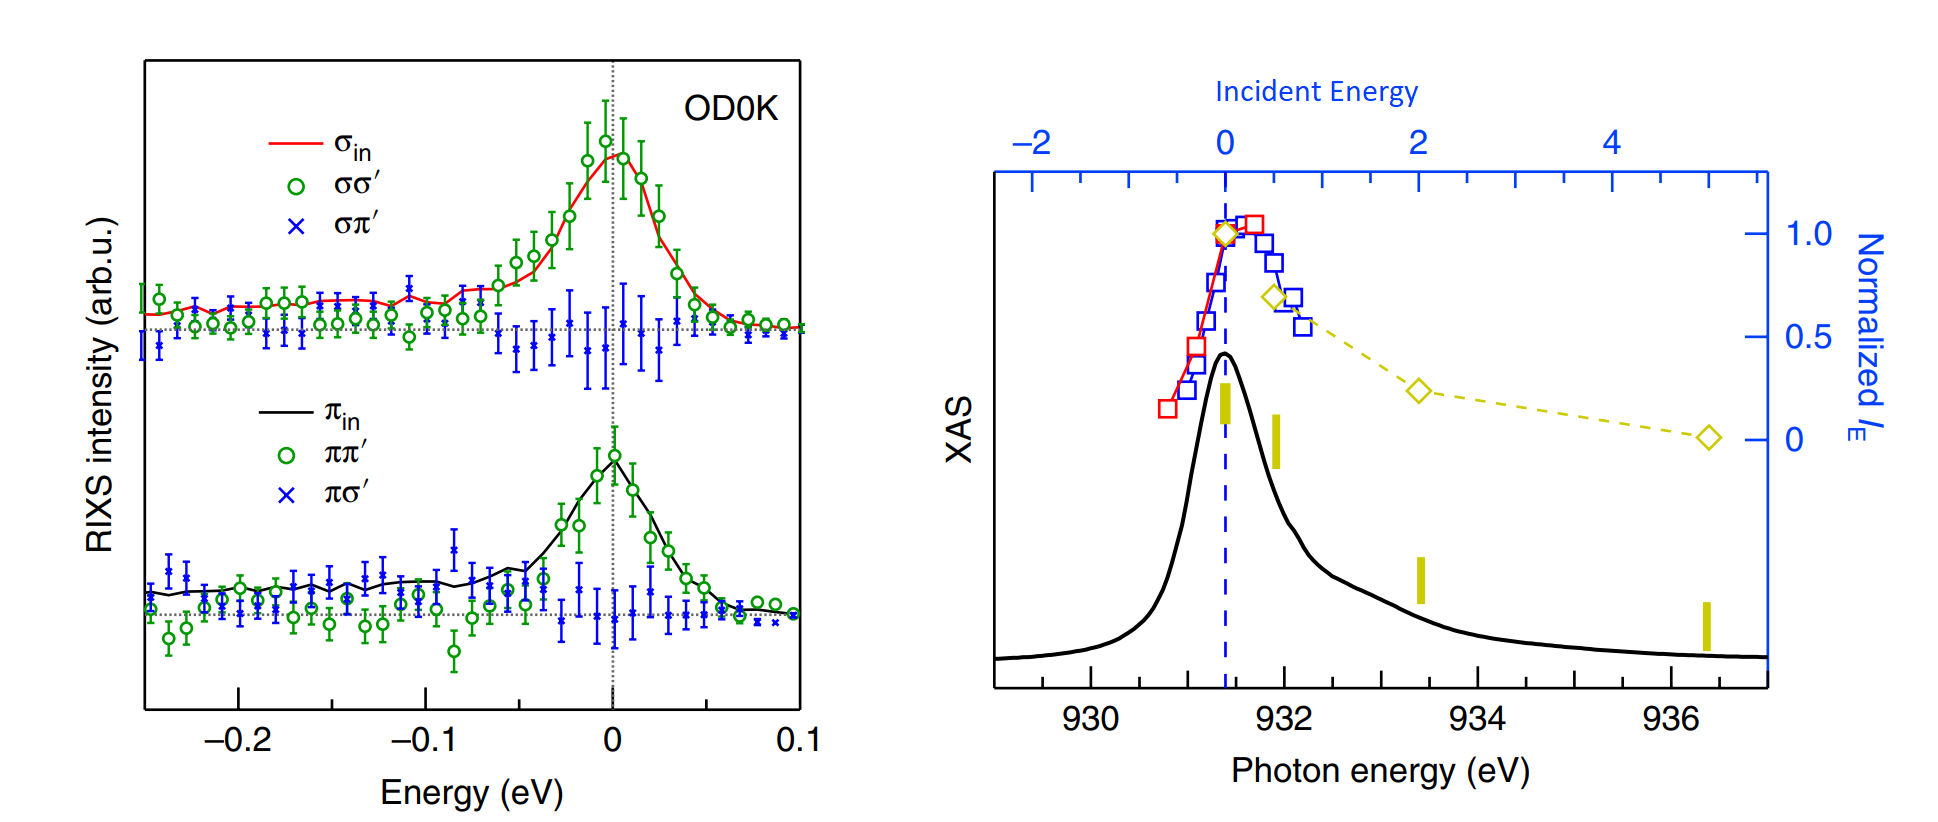
\includegraphics[width=4in]{figs/2018_2c_3a.png}
% \caption*{(\textbf{Left}) Polarization-resolved measurements for OD0K at $H = 0.115$. (\textbf{Right}) (Left and bottom axes) X-ray absorbtion spectrum of OD17K. (Right and top axes) Incident energy dependence of the REXS intensity}
% \end{figure}
% \end{frame}

% \begin{frame}{Doping dependence}
% \begin{itemize}
% \item The peak intensity is higher in the overdoped region
% \item The correlation lengths $\xi$ are comparable to LCO and YBCO
% \end{itemize}
% \begin{figure}
% 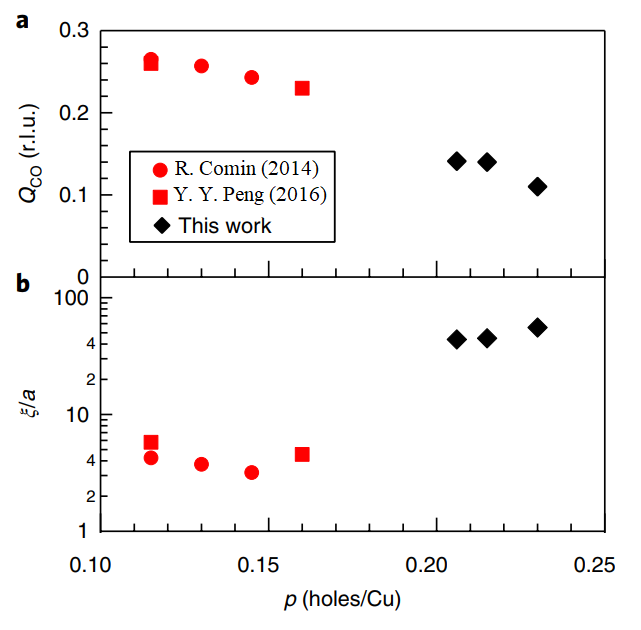
\includegraphics[width=2.5in]{figs/2018_4.png}
% \caption*{Doping dependence of $q_\text{CDW}$ (\textbf{a}) and correlation length (\textbf{b})}
% \end{figure}
% \end{frame}

% % not sure why they didn't do overdoped in previously
% % they call this peak REXS

% \begin{frame}{Need to revisit existing theories}
% \begin{itemize}
% \item Charge instabilities are related to the van Hove singularity and Fermi surface nesting, (which are absent in this experiment)
% \item CDWs arise from the pseudogap phase (relevant to only the underdoped region)
% \end{itemize}
% \end{frame}

% \begin{frame}{Summary}
% \begin{itemize}
% \item CDW can exist well above optimal doping
% \end{itemize}
% \end{frame}

% \begin{frame}{Why care about the Fermi surface (FS)?}
% \begin{itemize}
%   \item The origins of various phenomena can be traced back to the FS shape
%   \item Helps understand the mechanism of charge density waves
%   \item Can be experimentally measured
%   % \item

%   % \item The Fermi surface is the surface in reciprocal space which separates occupied from unoccupied electron states at zero temperature


% % \item CDW is a phase transition at low $T$
% % \item Metals undergo a phase transition when they are cooled
% % \item i.e. Iron and nickel become FM. Lead and Al become superconductors
% % \item Since 1970s, many layered materials have been found to undergo this phase transition
% % \item Want to study CDW
% \end{itemize}
% \end{frame}

% \begin{frame}{How to calculate the FS}
% \begin{itemize}
% \item Calculate the band structure using some method (by hand, tight binding, DFT, HF, etc.)
% \item Know the Fermi energy, $E_F$, from the number of electrons
% \item FS is a plot of constant energy with $E = E_F$
% \end{itemize}
% \end{frame}

% \begin{frame}{1D Fermi gas}
% \begin{itemize}
% \item The Fermi energy is given by
% \begin{align}
% E_F = \frac{\hbar^2}{2 m}\left(\frac{\pi n_F}{L}\right)^2 = \frac{\hbar^2}{2 m}\left(\frac{\pi N}{2 L}\right)^2,
% \end{align}
% because orbitals must be filled up to $n_F$ for $N$ electrons given by
% \begin{align}
% N = 2 \times \frac{1}{2} \times 2 n_F = 2 n_F,
% \end{align}
% where $n_F$ is the radius of an integer-space ``sphere''.
% \item The Fermi surface is points at $\pm \pi N / 2 L$
% \end{itemize}
% \end{frame}

% \begin{frame}{This FS geometry leads to a divergent response}
% \begin{itemize}
% \item The rearrangement of the charge density in a potential $\phi(\vf{r})$ can be written as
% \begin{align}
% \rho(\vf{q}) = \chi(\vf{q}) \phi(\vf{q}),
% \end{align}
% where $\chi(\vf{q})$ is the Lindhart function given in $d$ dimensions by
% \begin{align}
% \chi(\vf{q}) = \frac{1}{(2 \pi)^d} \int \frac{f_k - f_{k + q}}{E_k - E_{k + q}} d \vf{k},
% \end{align}
% which in the 1D case, evaluates to
% \begin{align}
% \chi(q) = \frac{k_F}{\pi E_F q}\ln{\left|\frac{q + 2k_F}{q - 2k_F}\right|}.
% \end{align}
% \end{itemize}
% \end{frame}

% \begin{frame}{An external perturbation leads to a divergent charge density}
% \begin{itemize}
% \item Causes a charge density redistribution
% \item The divergence at $q = 2 k_F$ is called \textbf{perfect nesting}
% \begin{figure}
% 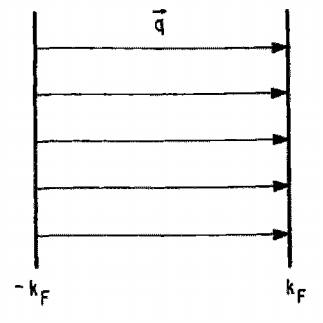
\includegraphics[width=1.5in]{figs/1d_nesting.png}
% \caption{\label{fig:1d_nesting} Fermi surface topology for a 1D electrong gas, The arrows indicate pairs of states, differing by the
% wavevector $q = 2 k_F$.}
% \end{figure}
% \end{itemize}
% \end{frame}

% \begin{frame}{The rearrangement of atoms and charges results in a lower energy}
% \begin{itemize}
% \item The new lattice has a period of $2a$
% \item The $\vf{k}$ vector now range from $-\pi / 2a$ to $\pi / 2a$
% \item The band is now split into two bands
% \item The atomic motion is causing the electrons to reconfigure
% \item This is called a \textbf{charge density wave (CDW)}
% \begin{figure}
% 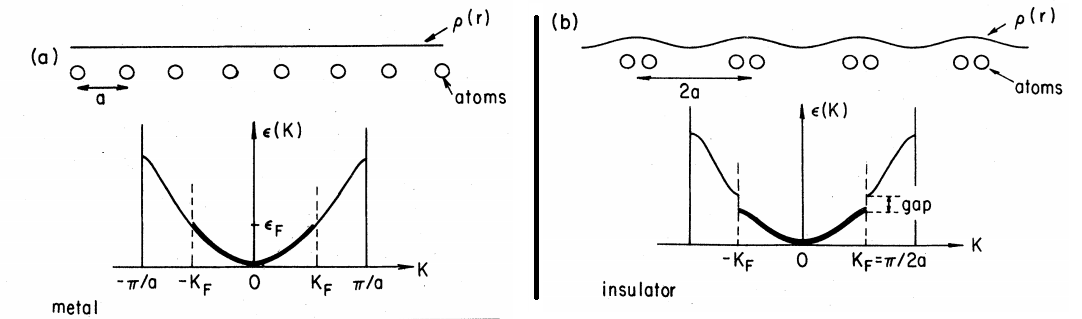
\includegraphics[width=3.5in]{figs/gap.png}
% \caption{\label{fig:gap} Peierls distortion in a one-dimensional metal with a half-filled band: (a) undistorted metal, (b) Peierls insulator.}
% \end{figure}
% % Imagine a line of atoms on equally-spaced positions sharing their electrons to make a conduction band.
% % You have exactly one electron per atom.
% % And, the k-vectors range from −π/a to π/a.
% %% The electrons are split in spin 50/50, so you get filling of the states in the first band up to exactly ±π/2a, and that's the Fermi surface (two points). This is called a half-filled band, since the states are filled duplicately until the exact half-way point.
% % But if there's electron-electron or electron-phonon interaction
% % period of the lattice is given by lambda = pi / k_F
% \end{itemize}
% \end{frame}

% \begin{frame}{What about superconductivity (SC)?}
% \begin{itemize}
% \item In 1954, Fröhlich attempted to explain SC using CDW (even before the BCS theory)
% \item His model was not wrong but incomplete (did not explain the Meissner effect)
% \item SC occurs in proximity to CDW
% \item Question: Is this significant (SC emerges from CDW) or trivial (the electronic structure independently favors both)?
% \end{itemize}
% \end{frame}

% \begin{frame}{Evidence of the competition between SC and CDW}
% \begin{itemize}
% \item J. Chang et al's \textit{Direct observation of competition between superconductivity and charge density wave order in YBa$_2$Cu$_3$O$_{6.67}$} (2012)
% \item Want to measure when such states exist
% \item X-ray diffration in magnetic fields up to 17~T with the hole concentration per Cu $p = 0.12$
% \end{itemize}
% \end{frame}

% \begin{frame}{Results: The CDW signal increases when SC is suppressed at $H = 17~T$ and $T = 2~K$}
% \begin{itemize}
% \item The charge modulation has two field- and temperature-independent wave vectors $\vf{q}_{\text{CDW}} = \vf{q}_1 = (\delta_1, 0, 0.5)$ and $\vf{q}_2 = (0, \delta_2, 0.5)$ where $\delta_1 = 0.305$ and $\delta_2 = 0.315$
% % \item The CDW gives rise to peaks the at $\vf{Q} = (2 \pm \delta_1, 0, 0.5)$
% \end{itemize}
% \begin{figure}
% 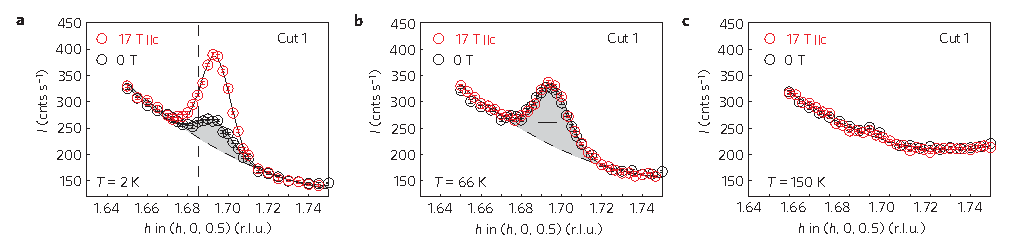
\includegraphics[width=\textwidth]{figs/chang_1.pdf}
% \caption{\label{fig:chang_1} Scans along $(h, 0, 0.5)$ for temperature and magnetic fields: (a) $T < T_c$, (b) $T_c < T < T_{\text{CDW}}$, (c) $T > T_{\text{CDW}}$}
% \end{figure}
% \end{frame}

% \begin{frame}{The FS of YBCO consists of bonding and anti-bonding sheets (according to ARPES and LDA)}
% \begin{itemize}
% \item The electronic states connected by $\vf{q}_{\text{CDW}}$ are the bonding bands near the zone boundary
% \item The states lie near the maxima of the superconducting gap
% \item This (probably) means the CDW state is competing with SC for FS
% \begin{figure}
% 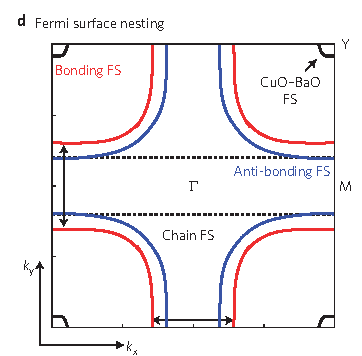
\includegraphics[width=1.5in]{figs/chang_3.pdf}
% \caption{\label{fig:chang_3} FS of YBCO}
% \end{figure}
% \end{itemize}
% \end{frame}

% \begin{frame}{Implications for the phase diagrams}
% \begin{itemize}
% \item A Landau theory: $T_c$ is suppressed in the presence the CDW
% \item $T_{\text{CDW}}$ corresponds with $T_\text{H}$, where Hall effect measurements suggest FS reconstruction
% \item A CDW that breaks translational symmetry explains the mechanism of FS reconstruction
% \end{itemize}
% \begin{figure}
% \includegraphics[width=1.5in]{figs/chang_4.pdf}
% \caption{\label{fig:chang_4} Doping dependence of several ordering temperatures}
% \end{figure}
% \end{frame}

% \begin{frame}{Conclusion}
% \begin{itemize}
% \item The Fermi surface nesting results in a diverging charge distribution
% \item The atomic distortion and electron rearrangement to the lower energy are called \textbf{charge density wave}
% \item The charge density wave signal increases when the superconductivity is suppressed
% \end{itemize}
% \end{frame}

% \begin{frame}{Peierls' picture: 1D chain}
% \begin{itemize}
% % \item In 1930s, Peierls described the instability in a 1D chain of equally spaced atoms
% % \item The only zero energy transition is from $k_F$ to $-k_F$, % where $k_F$ is the Fermi wave number
% \item The Fermi points are at $k_F = \pm \pi / 2 a$ % connected by a vector $q = 2 k_F$
% % \item The disturbance with $q = 2 k_F$ changes spacing to $2 a$
% \item Gap occurs at $k = \pm \pi / 2 a$ when $T < T_c$
% \item Metal-to-insulator transition at $T_c$ is called \textbf{Peierls' transition}

% \end{itemize}
% \end{frame}

% \begin{frame}{Free electron gas model}
% \begin{itemize}
% \item \textbf{Lindhard response function} $\chi(q)$ describes free electron gas' response
% \item 1D electron gas is unstable
% % \begin{figure}
% % 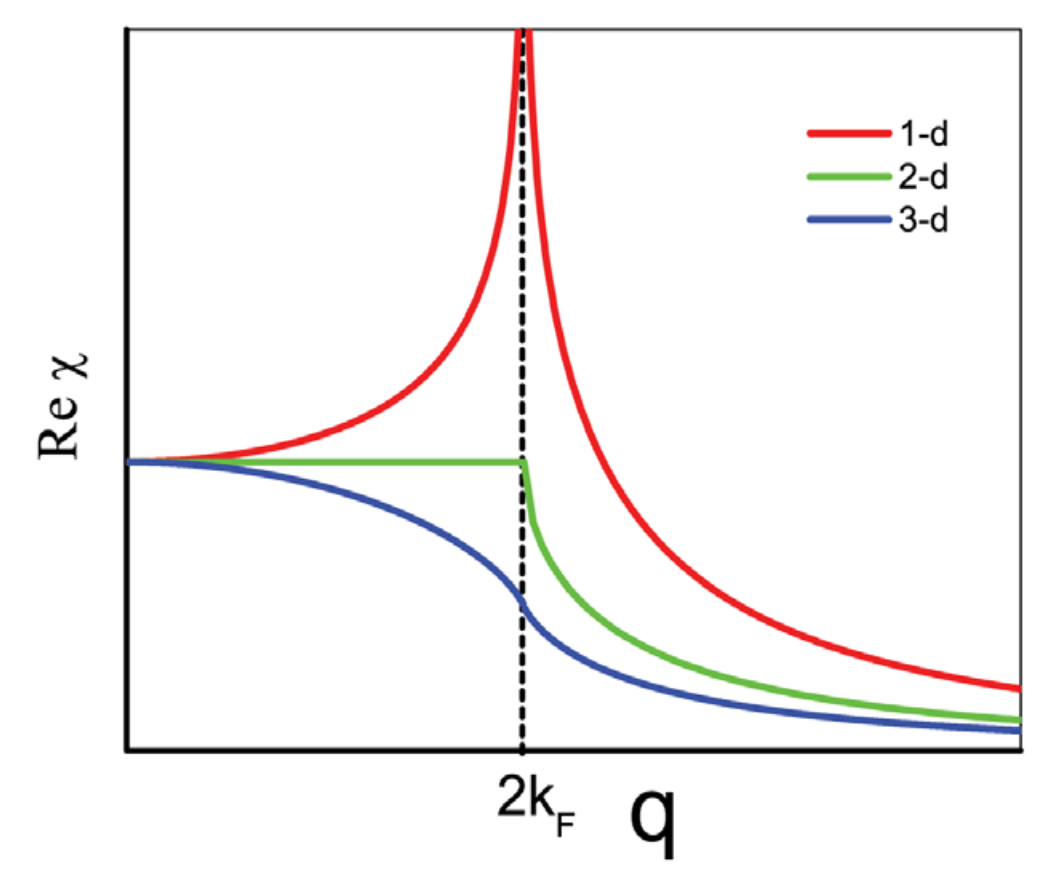
\includegraphics[width=2.5in]{figs/lindhart.png}
% % \caption{\label{fig:lindhart} Real part of Linhard function for 1D, 2D and 3D free electron gas models}
% % \end{figure}
% \end{itemize}
% \end{frame}

% \begin{frame}{Kohn anomaly}
% \begin{itemize}
% \item In 1959, Kohn: The excitations at $2 k_F$ will screen any lattice motion with this wave vector
% \item The phonon modes near $2 k_F$ will drop to a lower energy
% \item This is called \textbf{phonon softening}
% %  This strong renormalization of the phonon due to interactions with an electron system is referred to as the Kohn anomaly
% % \begin{figure}
% % 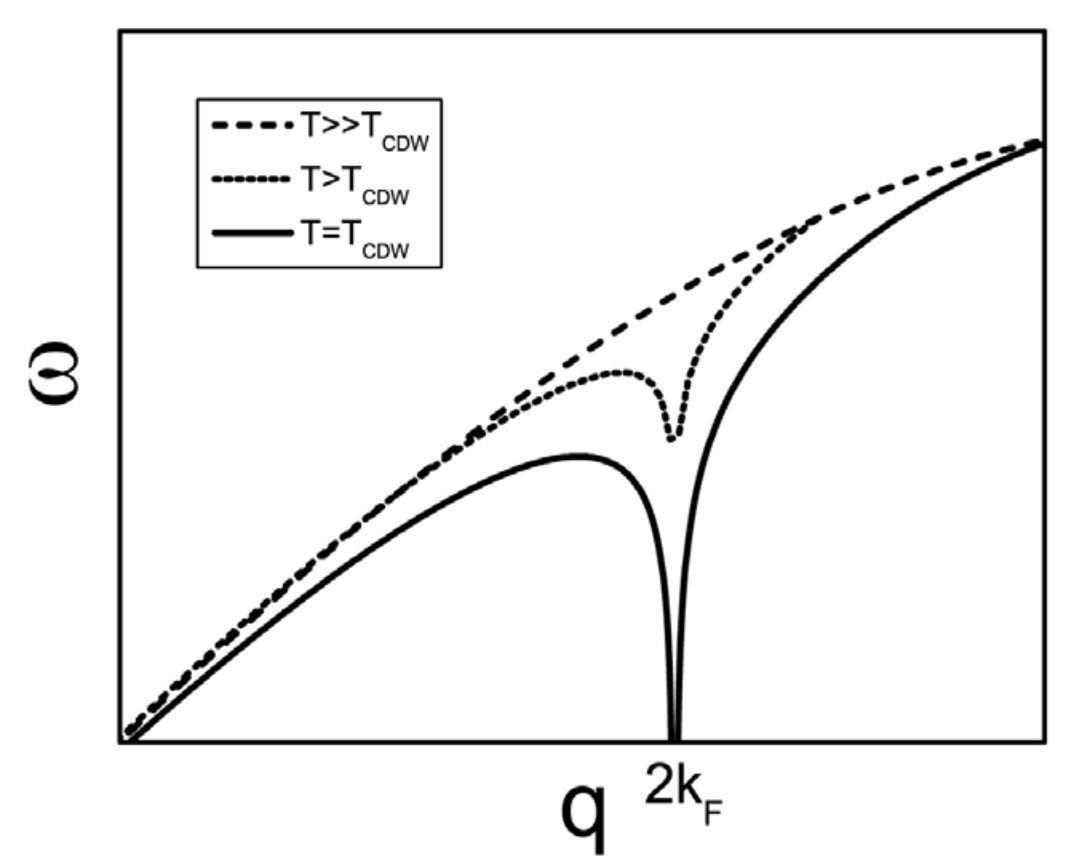
\includegraphics[width=2in]{figs/kohn_anomaly.png}
% % \caption{\label{fig:kohn_anomaly} Phonon energy of 1D chain at different $T$}
% % \end{figure}
% \end{itemize}
% \end{frame}

% \begin{frame}{Miao and Dean's \textit{Incommensurate Phonon Anomaly and the Nature of Charge Density Waves in Cuprates} (2018)}
% \begin{itemize}
% \item \textit{Goal:} Find unifying description for superconducting cuprates
% \item CDW instabilities are common superconducting cuprates
% \item CDWs have different ordering wave vectors
% \item They measured the $T$ dependence of the low-energy phonons in La$_{1.875}$Ba$_{0.125}$CuO$_4$ and compared it to YBa$_2$Cu$_3$O$_{6 + \delta}$
% \end{itemize}
% \end{frame}

% \begin{frame}{Inelastic x-ray scattering measurement of $S(\vf{Q}, \omega)$}
% \begin{itemize}
% \item Why measured $S(\vf{Q}, \omega)$? ``Because they can" - Lucas
% % \item Dashed lines are calculated using DFPT with PBE functional
% % \begin{figure}
% % 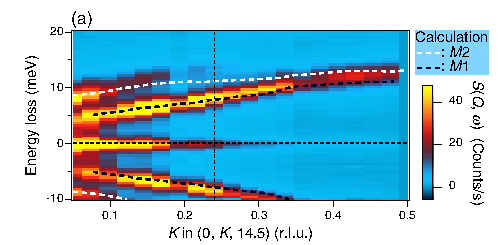
\includegraphics[width=3.5in]{figs/exp_sq.pdf}
% % \caption{\label{fig:exp_sq} Phonon dynamic structure factor at $T = 300~\mathrm{K}$}
% % \end{figure}
% \end{itemize}
% \end{frame}

% \begin{frame}{Example fits of spectra at $K$ = 0.09, 0.23, and 0.31 r.l.u. at different $T$}
% % \begin{figure}
% % 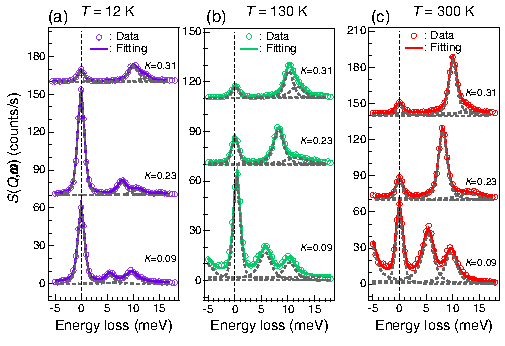
\includegraphics[width=3.5in]{figs/exp_fit.pdf}
% % \caption{\label{fig:exp_fit} }
% % \end{figure}
% \end{frame}

% \begin{frame}{Peaks at different $T$}
% % \begin{figure}
% % 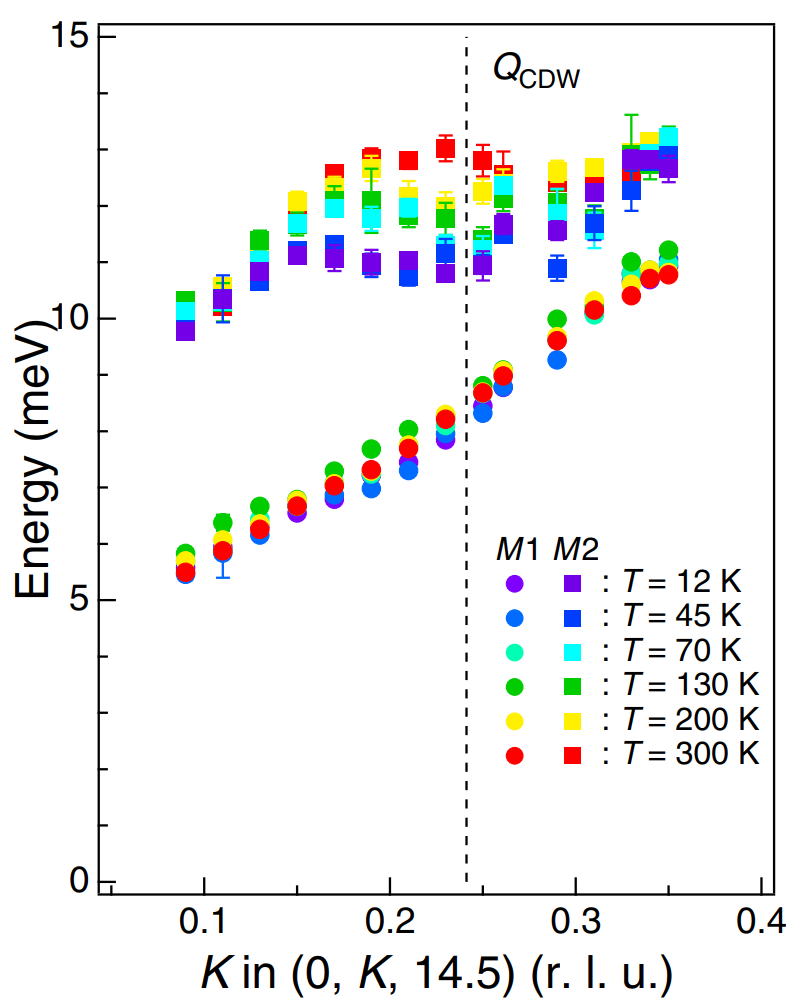
\includegraphics[width=2.2in]{figs/exp_E_k.png}
% % \caption{\label{fig:exp_E_k} $Q_{\text{CDW}} = 0.23~\mathrm{r.l.u.}$}
% % \end{figure}
% \end{frame}

% \begin{frame}{$T$ dependence at $K = 0.23~\mathrm{r.l.u.}$}
% \begin{itemize}
% \item Since they found that $M2$ has a large component of $c$-axis displacements, they suggest that $c$-axis coupled most strongly to the CDW
% % \begin{figure}
% % 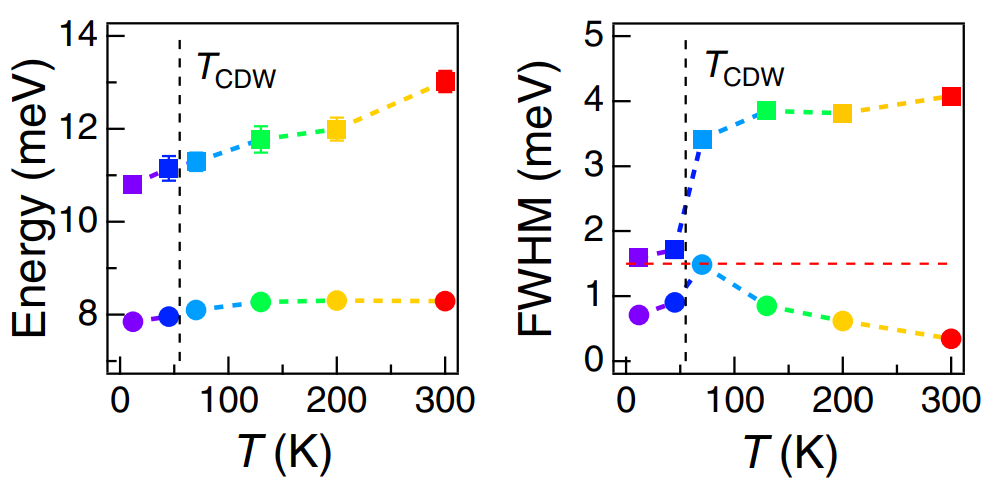
\includegraphics[width=3.5in]{figs/exp_T_dependence.png}
% % \caption{\label{fig:exp_T_dependence} $T_{\text{CDW}} = 55~\mathrm{K}$}
% % \end{figure}
% \end{itemize}
% \end{frame}

% \begin{frame}{Maximum phonon softening moves with increasing $T$}
% \begin{itemize}
% \item They conclude that $Q_{\text{CDW}} = 0.238~\mathrm{r.l.u.}$ at $T = 55~\mathrm{K}$, and $Q_{\text{CDW}} = 0.3~\mathrm{r.l.u.}$ at $T = 300~\mathrm{K}$
% \item Which is similar to a wave vector reported in YBa$_2$Cu$_3$O$_{6 + \delta}$
% % \begin{figure}
% % 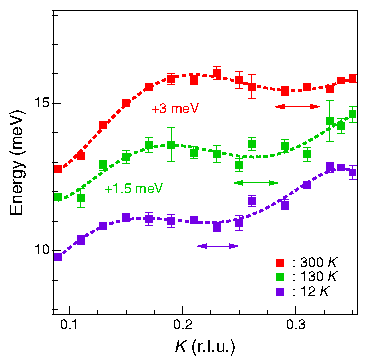
\includegraphics[width=2.5in]{figs/exp_E_k_zoomed.pdf}
% % \caption{\label{fig:exp_E_k_zoomed} }
% % \end{figure}
% \end{itemize}
% \end{frame}

% \begin{frame}{My research}
% \begin{itemize}
% \item \textit{Goal:} Identify phonon-softening modes of charge density waves in \ce{SrCuO2} and \ce{La2CuO4}???
% \item Step 1: Optimize the geometry of undoped and 1/4-doped \ce{SrCuO2} using DFT with 2x2 unit cells and PBEsol functional
% \item Step 2: Find phonon frequencies and eigenvectors at the gamma point
% \end{itemize}
% \end{frame}

% \begin{frame}{Identify how modes change after doping}
% \begin{itemize}
% \item The matrix element of $i$th AFM mode and $j$th Flip mode
% \begin{align}
% e_{ij} = \sum_{k = 1}^{48} v_{\text{AFM}, ik} \times v_{\text{Flip}, jk}
% \end{align}
% \item The two modes whose dot product is more than 0.8 are consider to be the same
% \begin{table}
% % \centering
% % \caption{\label{tab:dot} Dot products of  \ce{SrCuO2} (normallized within each column)}
% % \caption{\label{tab:widgets}Example values of the magnetic susceptibility, $\chi_v$.}
% \begin{tabular}{ccccccccccc}
% AFM / Flip & 1 & 2 & 3 & 4 & 5 & 6 & 7 & 8 & 9 & 10 \\
% % \colrule \\
% 1 & 0 & 0 & 0.895 & 0 & 0 & 0 & 0 & 0 & 0 & 0 \\
% 2 & 0.895 & 0 & 0 & 0 & 0 & 0 & 0 & 0 & 0 & 0 \\
% 3 & 0 & 0.875 & 0 & 0 & 0 & 0 & 0.001 & 0 & 0 & 0.047 \\
% 4 & 0 & 0 & 0 & 0.805 & 0 & 0 & 0 & 0 & 0 & 0 \\
% 5 & 0 & 0 & 0 & 0 & 0.806 & 0 & 0 & 0 & 0 & 0 \\
% 6 & 0 & 0 & 0 & 0 & 0 & 0 & 0 & 0 & 1.000 & 0 \\
% \end{tabular}
% \end{table}
% \end{itemize}
% \end{frame}

% \begin{frame}{The change in phonon frequency}
% % \begin{figure}
% % 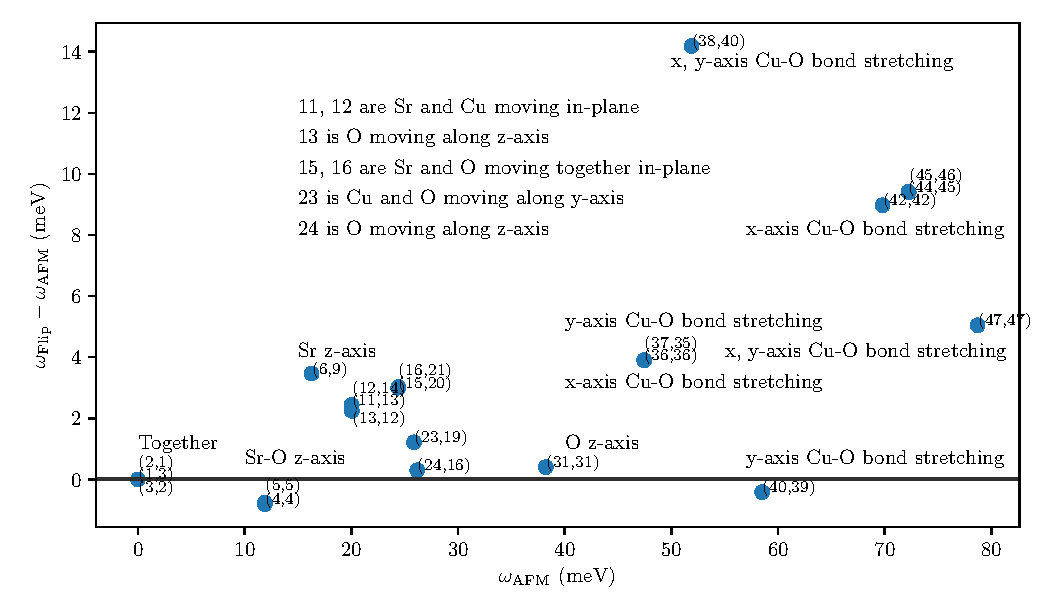
\includegraphics[width=4.2in]{figs/sco_afm_flip_freq.pdf}
% % \caption{\label{fig:sco_afm_flip_freq} See AVI files}
% % \end{figure}
% \end{frame}

% \begin{frame}{Conclusion}
% \begin{itemize}
% \item Kohn: Charge density waves affect phonon frequencies
% \item Dean: CDW in LCO and YBCO might be of the same origin (they both have $Q_{\text{CDW}} = 0.3~\mathrm{r.l.u.} at T = 300~\mathrm{K}$)
% \item My research: Doping weakens the Sr-O and Cu-O bonds
% \end{itemize}
% \end{frame}

\end{document}
